\documentclass[12pt,a4paper]{article}
\usepackage[paper=a4paper]{geometry}% http://ctan.org/pkg/geometry
\usepackage[english]{babel}
\usepackage[T1]{fontenc}


\usepackage{fancyvrb}
\usepackage{multicol}
\usepackage{lipsum}
\usepackage{setspace}
\usepackage{soul}
\usepackage{fontspec}
 \usepackage{colortbl}
\usepackage{background}
\usepackage{caption}
\usepackage{pgfgantt}
\usepackage{graphicx}
\usepackage[yyyymmdd]{datetime}
\usepackage{tikz}
\usetikzlibrary{calc}
\usepackage{indentfirst} 
\usepackage{pgfgantt}
\usepackage{rotating}
\usepackage[graphicx]{realboxes}
\usepackage{tocloft}
\usepackage{xcolor}
\usepackage{listings}

\definecolor{mGreen}{rgb}{0,0.6,0}
\definecolor{mGray}{rgb}{0.5,0.5,0.5}
\definecolor{mPurple}{rgb}{0.58,0,0.82}
\definecolor{backgroundColour}{rgb}{0.95,0.95,0.92}

\lstdefinestyle{CStyle}{
    backgroundcolor=\color{backgroundColour},   
    commentstyle=\color{mGreen},
    keywordstyle=\color{magenta},
    numberstyle=\tiny\color{mGray},
    stringstyle=\color{mPurple},
    basicstyle=\footnotesize,
    breakatwhitespace=false,         
    breaklines=true,                 
    captionpos=b,                    
    keepspaces=true,                 
    numbers=none,                    
    numbersep=5pt,                  
    showspaces=false,                
    showstringspaces=false,
    showtabs=false,                  
    tabsize=2,
    language=C
}



\newcommand{\listappendicesname}{Appendices}
\newlistof{appendices}{apc}{\listappendicesname}
\newcommand{\appendices}[1]{\addcontentsline{apc}{appendices}{#1}}

\newcommand{\newappendix}[1]{\section*{#1}\appendices{#1}}


\usepackage{sectsty}
\usepackage{float}
%\usepackage[table,xcdraw]{xcolor}
\sectionfont{\fontsize{24pt}{36}\selectfont}
\usepackage{tocloft}
\renewcommand{\cftsecleader}{\cftdotfill{\cftdotsep}}
\usepackage{afterpage}

\usepackage{listings}
\usepackage{color}
 
\definecolor{codegreen}{rgb}{0,0.6,0}
\definecolor{codegray}{rgb}{0.5,0.5,0.5}
\definecolor{codepurple}{rgb}{0.58,0,0.82}
\definecolor{backcolour}{rgb}{0.95,0.95,0.92}
 
\lstdefinestyle{mystyle}{
    backgroundcolor=\color{backcolour},   
    commentstyle=\color{codegreen},
    keywordstyle=\color{magenta},
    numberstyle=\tiny\color{codegray},
    stringstyle=\color{codepurple},
    basicstyle=\footnotesize,
    breakatwhitespace=false,         
    breaklines=true,                 
    captionpos=b,                    
    keepspaces=true,                 
    numbers=left,                    
    numbersep=5pt,                  
    showspaces=false,                
    showstringspaces=false,
    showtabs=false,                  
    tabsize=2
}
 
\lstset{style=mystyle}
\captionsetup{justification=raggedright,singlelinecheck=false}

\newcommand\blankpage{%
    \null
    \thispagestyle{empty}%
    \addtocounter{page}{-1}%
    \newpage}
\renewcommand{\baselinestretch}{1.5} 

\usetikzlibrary{calc}
\newcommand\HRule{\rule{\textwidth}{1pt}}

\setmainfont[Ligatures=TeX]{Times New Roman}
\newgeometry{top=20mm,bottom=20mm,left=28mm,right=13mm}
\usepackage[citestyle=reading]{biblatex}
\addbibresource{report.bib}

\backgroundsetup{
color=black,
scale=1,
opacity=1,
angle=0,
contents={
\begin{tikzpicture}
\draw [line width=0.75pt] ($ (current page.north west) + (2.5cm,-1cm) $) rectangle ($ (current page.south east) + (-1cm,1cm) $);
\draw [line width=0.01pt] ($ (current page.north west) + (0cm,0cm) $) rectangle    ($ (current page.south east) + (0cm,0cm) $); 
\end{tikzpicture}
}
}

\setlength{\footskip}{20pt}


\begin{document}

\begin{titlepage}

\begin{flushright}
\textbf{\uppercase{\fontsize{12}{18} \selectfont {Group No: E2}}}
\end{flushright}


\center % Center everything on the page
{\setstretch{1.2}

\includegraphics[width=2in,height=2in,keepaspectratio]{logo.png}\\[0.5cm]
\fontsize{16pt}{24}\selectfont \textbf{Project Report}\\[0.5cm]
\fontsize{16pt}{24}\selectfont \textbf{EGT 31303}\\[0.75cm]
\fontsize{24pt}{30}\selectfont \textbf{\uppercase{Digital Measuring System for Cloth}}\\[1.5cm]
\fontsize{16pt}{24}\selectfont \textbf{By}\\[0.5cm]
\fontsize{12pt}{12}\selectfont {
\bgroup
\def\arraystretch{2}% 
\begin{tabular}{|c|l|c|}
        \hline
        \textbf{Index No} &        \textbf{Name} &         \textbf{Marks} \\
        \hline
EGT/16/00025 &  Dissanayake HDSC & \\
        \hline
EGT/16/00037 & Gnanakeethan B & \\
        \hline
EGT/16/00042 & Hansa RYD & \\
        \hline
EGT/16/00051 & Imtiyaz FA & \\
        \hline
EGT/16/00061 & Kamalka HAB & \\
        \hline

\end{tabular}
\egroup
}


\vspace{1.5cm}
\fontsize{12pt}{12}\selectfont \textbf {Department of Engineering Technology \\ Faculty of Technology\\University of Sri Jayewardenepura\\ Sri Lanka}\\[0.5cm]
}

\vfill % Fill the rest of the page with whitespace

\end{titlepage}


\pagenumbering{roman}
\section{Abstract}

We have designed and developed a digital measurement system which can complement the existing solutions with ease. The digital system will enable users to be able to take measurements with single hand and easily note them down or save in their smartphones. 

\section{Acknowledgments}

In performing our assignment, we had to take the help and guideline of some respected persons, who deserve our greatest attitude. We would like to show our gratitude to Dr. Kanishka Madushanka for encouraging us to do such a innovation to get used with latest technologies and also to Mr.Isuru Udayanga for providing equipment and for facilitating.The completion of this assignment gives us much pleasure. And we like to expand our deepest gratitude to all colleagues those who have directly and indirectly guided us in constructing the instrument.


\newpage 
\renewcommand{\baselinestretch}{1}\normalsize
\tableofcontents
\renewcommand{\baselinestretch}{1.5}\normalsize

\listoffigures
 
\listoftables

\listofappendices

\newpage

\pagenumbering{arabic}
%\pagenumbering{gobble}
\setcounter{page}{1}
%\addcontentsline{toc}{section}{Unnumbered Section}


\section{Introduction}



	The purpose of this project was to design a measuring instrument to measure the length of cloths. We found that its realy hard to handle a meter ruler and cloth together while measuring.

At the garment sector this will be more usefull because as a third world country, the economy of the country is depend on garment field. This model can be used by the tailors too. We made this model as a rolling object. We can role the model on the cloth and then that displays the length of it. We got our inspiration from rolling meter ruler and tracing wheel.

The objectives of the project were:\\
�	To get a understanding of Arduino Project\\
�	To design a model with high precision\\
�	To get measurements with low effort\\
�	Work together as a group while making an innovation and helping group members to understand Arduino\\
�	The way of facing problems arose while working\\

This document provides background information and describes the tools used to build the model. As well, it explains the design methodology of the model and provides and explains simulation results. Finally, recommendations for others working on similar projects and for possible future work are provided.


\newpage
\section{Background Information}

\subsection{Design}
The prominence of simple ways to measure length is increasing as the public is lazy in this era. Therefore new and simple ways to measure lengths were created. In this technological era more precise and simple ways of measuring length, which include digital technology were created.
A simple diagram of the digital cloth measuring system is given below. Here the length is determined by the rotating disk. That disk has a radius of 2cm. which means that it has a circumference of nearly 12.56cm. The disk rotates the connected rotary encoder which has 30 division. This means when the encoder rotates its 1 division the length covered by the disk is 0.4 cm.
When the disk rolls on the cloth, the encoder rotates and gives the signal to the Arduino Nano and from there it gives an output to the display. A Switch is used to reset the readings.

\subsection{Instruments or Tools used}

\begin{itemize}
 	
\item	Quadrature encoder (with 30 divisions) [\cite[see Appendix]{ky40:2015}]\\
To design this model, we used KY-040 rotary encoder.
The Keyes KY-040 rotary encoder is a rotary input device (as in knob) that provides an indication of how much the knob has been rotated AND what direction it is rotating.


\item A disk (with a diameter of 4cm)
\item Arduino Nano v3( See Appendix 1)\\


\textbf{\underline{Powering:}}\\
There are totally three ways by which the Nano can power.\\
\textbf{USB Jack:} Connect the mini USB jack to a phone charger or computer through a cable and it will draw power required for the board to function�\\
\textbf{Vin Pin:} The Vin pin can be supplied with a unregulated 6-12V to power the board. The on-board voltage regulator regulates it to +5V\\
\textbf{+5V Pin:} If we have a regulated +5V supply then it can directly provide this to the +5V pin of the Arduino.\\
\textbf{\underline{Input/Output:}}

There are totally 14 digital Pins and 8 Analog pins on Nano board. The digital pins can be used to interface sensors by using them as input pins or drive loads by using them as output pins. A simple function like pinMode() and digitalWrite() can be used to control their operation. The operating voltage is 0V and 5V for digital pins. The analog pins can measure analog voltage from 0V to 5V using any of the 8 Analog pins using a simple function like analogRead()
These pins apart from serving their purpose can also be used for special purposes which are discussed below:
\begin{itemize}
\item \textbf{Serial Pins 0 (Rx) and 1 (Tx):} Rx and Tx pins are used to receive and transmit TTL serial data. They are connected with the corresponding ATmega328P USB to TTL serial chip.
\item \textbf{External Interrupt Pins 2 and 3:} These pins can be configured to trigger an interrupt on a low value, a rising or falling edge, or a change in value.
\item \textbf{PWM Pins 3, 5, 6, 9 and 11:} These pins provide an 8-bit PWM output by using analogWrite() function.
\item \textbf{SPI Pins 10 (SS), 11 (MOSI), 12 (MISO) and 13 (SCK):} These pins are used for SPI communication.

\item \textbf{In-built LED Pin 13:} This pin is connected with an built-in LED, when pin 13 is HIGH ? LED is on and when pin 13 is LOW, its off.
\item \textbf{I2C A4 (SDA) and A5 (SCL):} Used for IIC communication using Wire library.
\item \textbf{AREF:} Used to provide reference voltage for analog inputs with analogReference() function.
\item \textbf{Reset Pin:} Making this pin LOW, resets the microcontroller.
These special functions and their respective pins are illustrated in the Arduino Nano Pin Diagram shown below.
\end{itemize}



\item Output - 7-segment 4-character display [\cite[see Appendix]{display:2015}]
\\Seven-segment displays are used to display the digits in digital watches, calculators, clocks, measuring instruments and digital counters, etc. Generally, LCD and LED segments provide the display output of numerical numbers and characters.
\item A 9V battery
\item Jumper wires
\item Switch
\item A plastic container to assemble

\end{itemize}






\newpage
\begin{figure}[h]
    \centering
    \begin{minipage}{0.45\textwidth}
        \centering
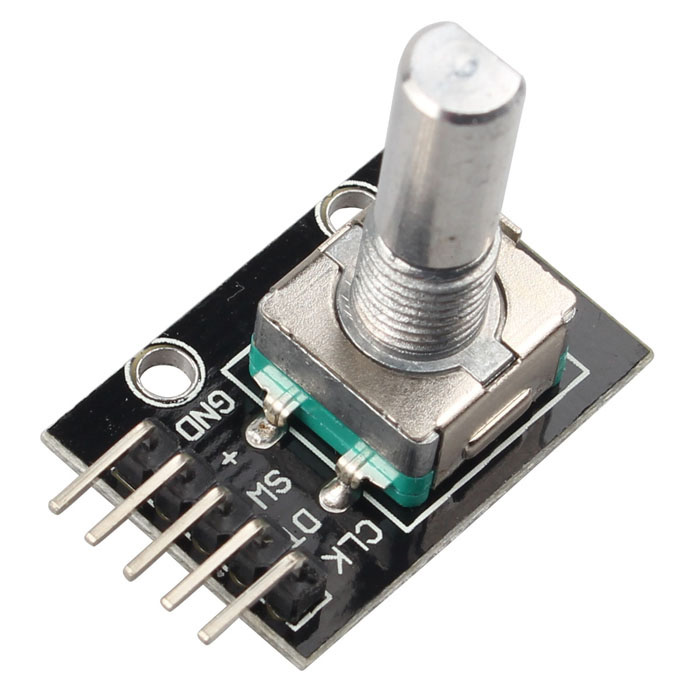
\includegraphics[width=0.5\textwidth]{ky040}
\caption{Quadrature Encoder}
    \end{minipage}\hfill
    \begin{minipage}{0.5\textwidth}
        \centering
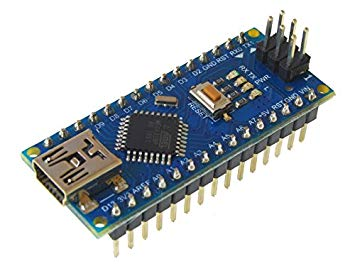
\includegraphics[width=0.5\textwidth]{arduino}
\caption{Arduino Nano V3}
    \end{minipage}
\end{figure}
\begin{figure}[h]
    \centering
    \begin{minipage}{0.45\textwidth}
        \centering
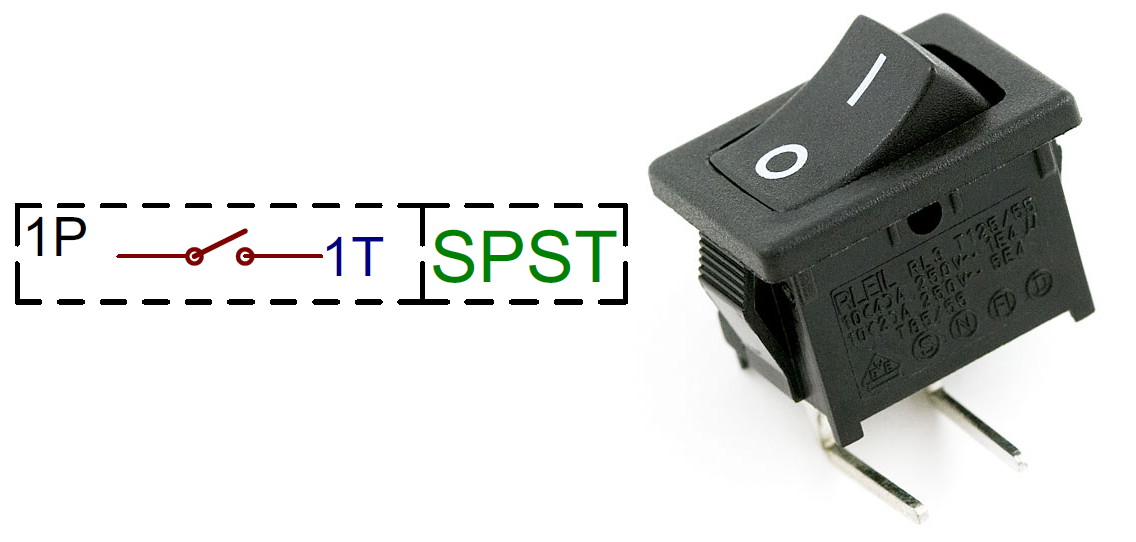
\includegraphics[width=0.5\textwidth]{switch}
\caption{SPST Switch}
    \end{minipage}\hfill
    \begin{minipage}{0.5\textwidth}
        \centering
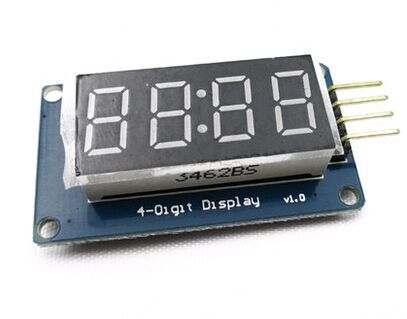
\includegraphics[width=0.5\textwidth]{TM1637}
\caption{4-Char 7 Segment Display}
    \end{minipage}
\end{figure}


\begin{figure}[h]
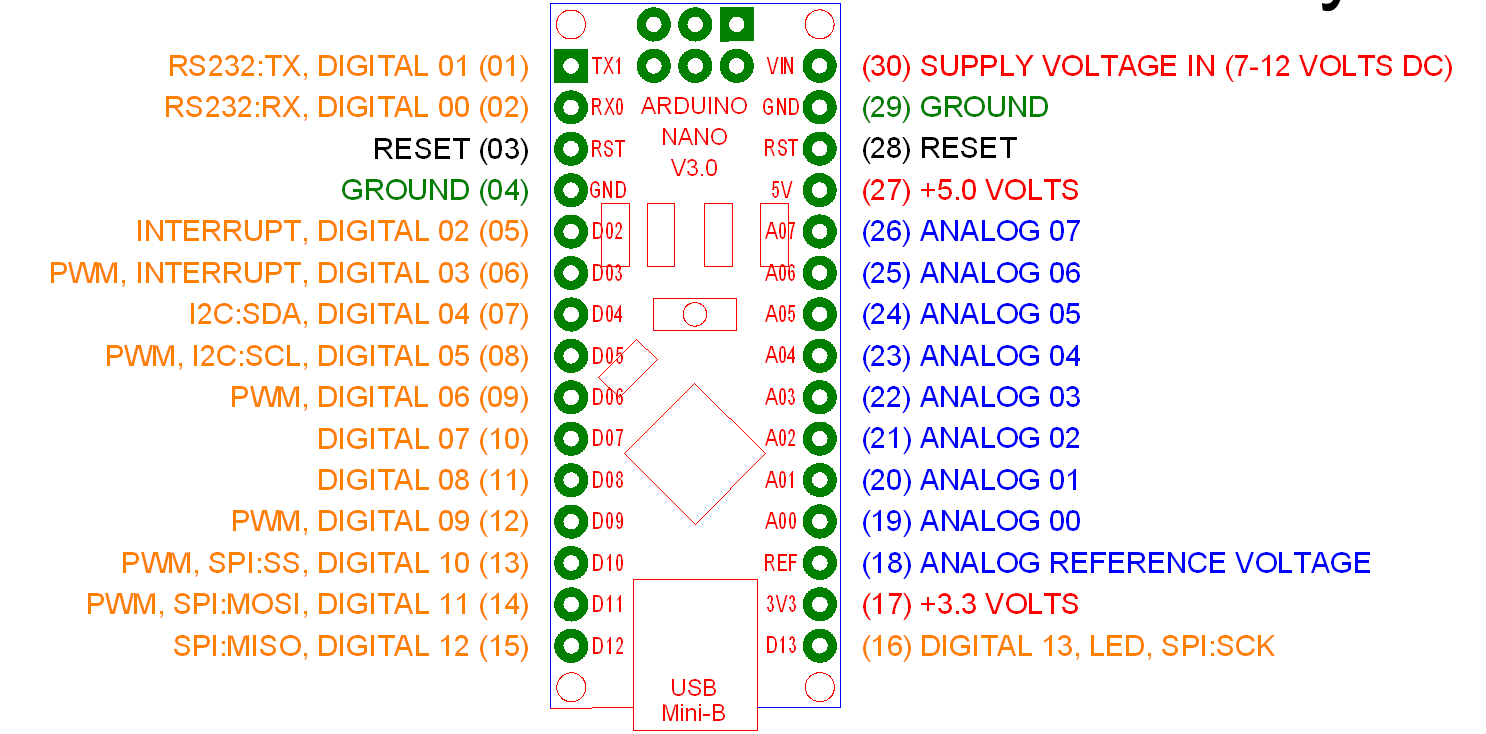
\includegraphics[width=1\textwidth]{pindiagram}
\caption{Arduino Nano Pin Diagram}
\end{figure}
\newpage



\section{Theory}


The working principle is based on Quadrature Encoder.The code disk inside a quadrature encoder contains two tracks usually denoted Channel A and Channel B. These tracks or channels are coded ninety electrical degrees out of phase, as indicated in the image below, and this is the key design element that will provide the quadrature encoder its functionality. In applications where direction sensing is required, a controller can determine direction of movement based on the phase relationship between Channels A and B. As illustrated in the figure below, when the quadrature encoder is rotating in a clockwise direction its signal will show Channel A leading Channel B, and the reverse will happen when the quadrature encoder rotates counterclockwise.

\begin{figure}[h]
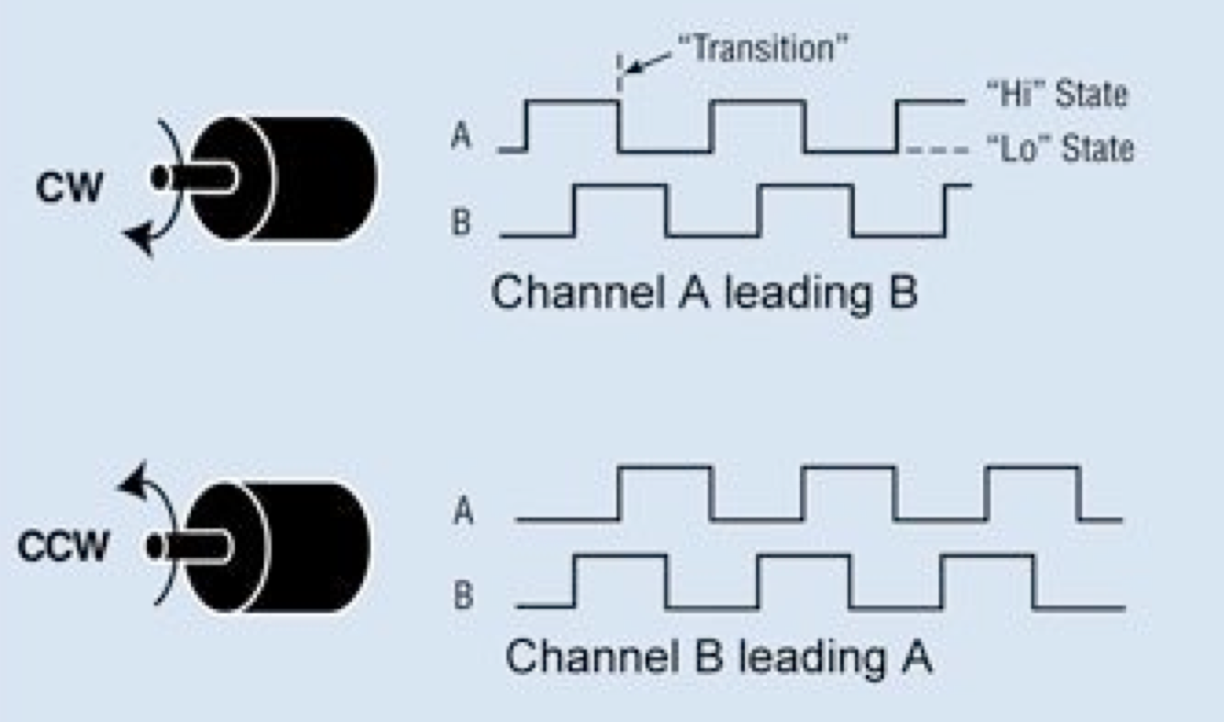
\includegraphics[width=0.5\textwidth]{encoder}
\caption{Quadrature Encoder}
\end{figure}


\section{ Design methodology}

The design is absolutely simplified to reduce costs. As a replacement for a meter-ruler, it must be cost-effective to manufacture and to the customer as well. It must be handy as well. Due to these reasons we decided on using a Arduino Nano and a 4-char 7-segment display.

Apart from direction, position can also be monitored with a quadrature encoder by producing another signal known as the "marker", "index" or "Z channel". This Z signal, produced once per complete revolution of the quadrature encoder, is often used to locate a specific position during a 360� revolution.

\section{ Block Diagram}
\begin{figure}[H]
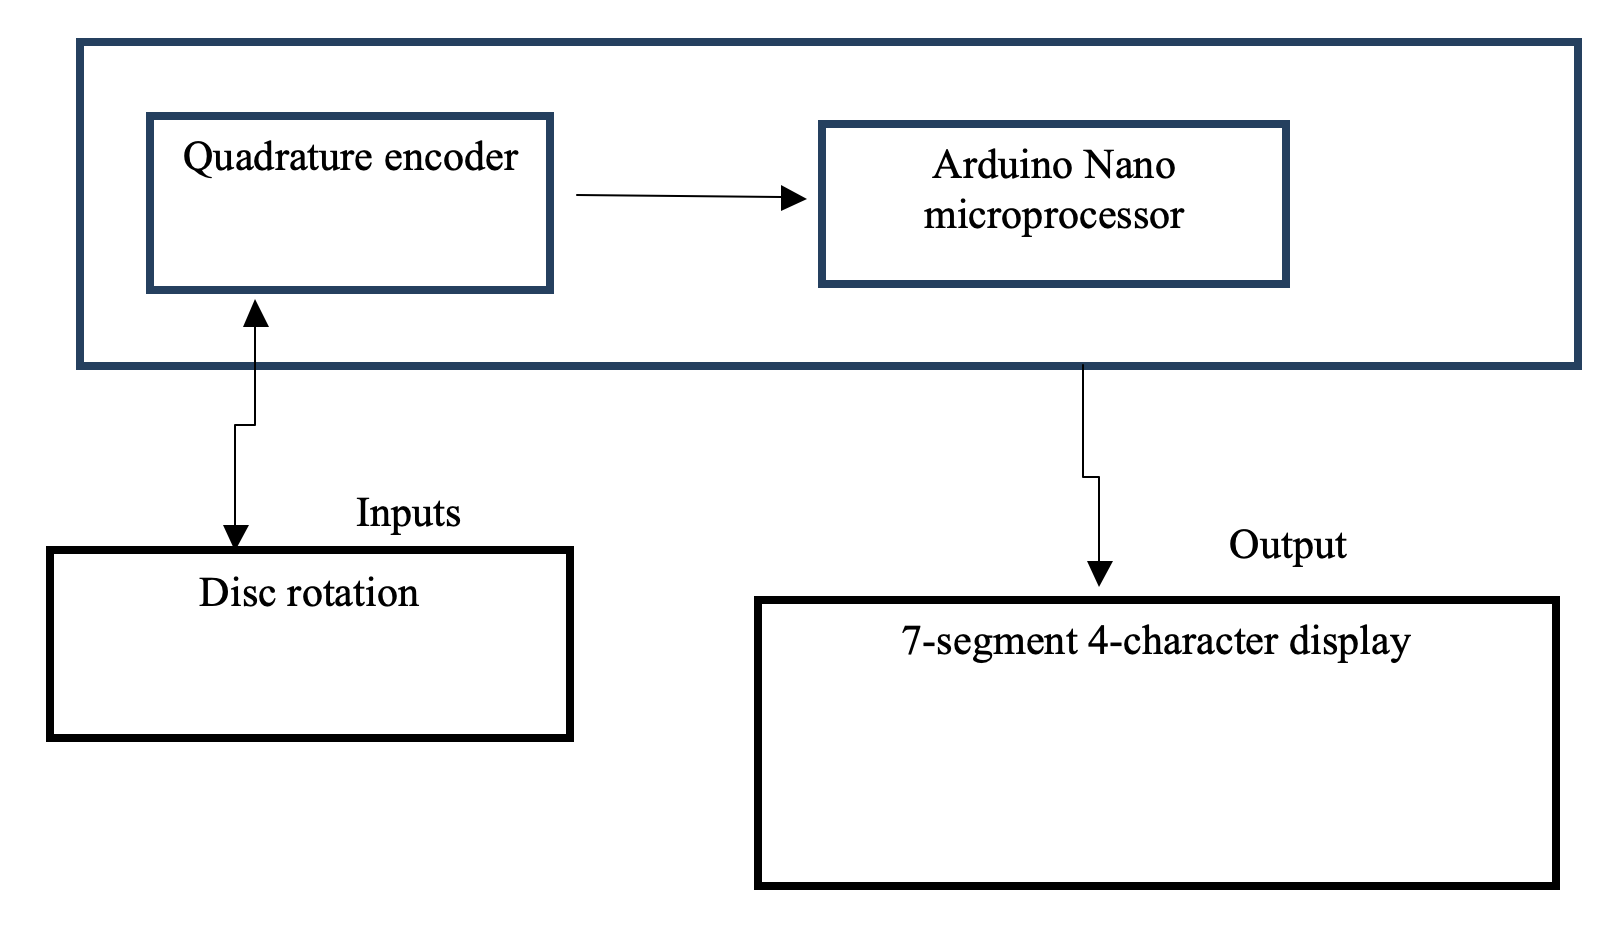
\includegraphics[width=0.9\textwidth]{blockdiagram}
\caption{Block Diagram}
\end{figure}


\section{Process}
\begin{itemize}
\item The instruments and tools were collected
\item The center of the disk was found and drilled
\item The disk was joined to the quadrature encoder 
\item The quadrature encoder was connected to the Arduino Nano
\item The code was uploaded to the Arduino Nano
\item The 7-segment 4-character display was connected and check for the errors.
\item The whole setup was set in to the container 
\end{itemize}
 \newpage 

\section{Conclusion and Recommendations}
\begin{itemize}
\item It could have been better if we could utilize a more-specific and accurate rotary sensor. 
\item It is possible to create A more-compact design
\item It is possible to develop a Android/iOS application which works over Bluetooth. 
\end{itemize}


\newpage
\newappendix{Appendix 1}

\begin{table}[H]
\centering
\caption{Arduino Nano Pin Configuration}

\arrayrulecolor{black}
\begin{tabular}{!{\color{black}\vrule}l!{\color{black}\vrule}l!{\color{black}\vrule}l!{\color{black}\vrule}} 
\hline
Pin Category        & Pin Name                                   & Details                                                                                                                                                                                                                                                                         \\ 
\hline
Power               & Vin, 3.3V, 5V,GND                          & 
\begin{minipage}[t]{0.5\columnwidth}%
Vin:~Input voltage to Arduino when using an external power source (6-12V).5V:~Regulated power supply used to power microcontroller and other components on the board.3.3V:~3.3V supply generated by on-board voltage regulator. Maximum current draw is 50mA.GND:~Ground pins. 
\end{minipage} \\ 
\hline
Reset               & Reset                                      & Resets the microcontroller.                                                                                                                                                                                                                                                     \\ 
\hline
Analog Pins         & A0 - A7                                    & Used to measure analog voltage in the range of 0-5V                                                                                                                                                                                                                             \\ 
\hline
Input/Output Pins   & Digital Pins D0 - D13                      & 
\begin{minipage}[t]{0.2\columnwidth}%

Can be used as input or output pins. 0V (low) and 5V (high)                                                                                                                                                                                                                     
\end{minipage}  

\\ 
\hline
Serial              & Rx,~Tx                                     & Used to receive and transmit TTL serial data.                                                                                                                                                                                                                                   \\ 
\hline
External Interrupts & 2, 3                                       & To trigger an interrupt.                                                                                                                                                                                                                                                        \\ 
\hline
PWM                 & 3, 5, 6, 9, 11                             & Provides 8-bit PWM output.                                                                                                                                                                                                                                                      \\ 
\hline
SPI                 &
\begin{minipage}[t]{0.2\columnwidth}%
 10 (SS), 11 (MOSI), 12 (MISO) and 13 (SCK) 
\end{minipage}  
 & Used for SPI communication.                                                                                                                                                                                                                                                     \\ 
\hline
Inbuilt LED         & 13                                         & To turn on the inbuilt LED.                                                                                                                                                                                                                                                     \\ 
\hline
IIC                 & A4 (SDA), A5 (SCL)                         & Used for Two Way communication.                                                                                                                                                                                                                                                 \\ 
\hline
AREF                & AREF                                       & To provide reference voltage for input voltage.                                                                                                                                                                                                                                \\
\hline
\end{tabular}
\arrayrulecolor{black}
\end{table}



\begin{table}[H]
\centering
\caption{Arduino Nano Specification}
\arrayrulecolor{black}
\begin{tabular}{!{\color{black}\vrule}l!{\color{black}\vrule}l!{\color{black}\vrule}} 
\hline
Microcontroller                       & ATmega328P - 8 bit AVR family microcontroller  \\ 
\hline
Operating Voltage                     & 5V                                             \\ 
\hline
Recommended Input Voltage for Vin pin & 7-12V                                          \\ 
\hline
Analog Input Pins                     & 6 (A0 -A5)                                    \\ 
\hline
Digital I/O Pins                      & 14 (Out of which 6 provide PWM output)         \\ 
\hline
DC Current on I/O Pins                & 40 mA                                          \\ 
\hline
DC Current on 3.3V Pin                & 50 mA                                          \\ 
\hline
Flash Memory                          & 32 KB (2 KB is used for Bootloader)            \\ 
\hline
SRAM                                  & 2 KB                                           \\ 
\hline
EEPROM                                & 1 KB                                           \\ 
\hline
Frequency (Clock Speed)               & 16 MHz                                         \\
Communication                         & IIC, SPI, USART                                \\
\hline
\end{tabular}
\arrayrulecolor{black}
\end{table}
\newpage


\newappendix{Appendix 2}


\begin{lstlisting}[style=CStyle]
#include <Arduino.h>
#include <TM1637Display.h>


//SENSOR PINS
#define outputA 3
#define outputB 2

//DISPLAY PINS
#define CLK 7
#define DIO 5


TM1637Display display(CLK, DIO);


int counter = 0;
int aState;
int aLastState;
int length;
float lengthm;
void setup() {
  pinMode (outputA, INPUT);
  pinMode (outputB, INPUT);

  Serial.begin (9600);
  // Reads the initial state of the outputA
  aLastState = digitalRead(outputA);
}
void loop() {
  aState = digitalRead(outputA); // Reads the "current" state of the outputA
  // If the previous and the current state of the outputA are different, that means a Pulse has occured
  if (aState != aLastState) {
    // If the outputB state is different to the outputA state, that means the encoder is rotating clockwise
    if (digitalRead(outputB) != aState) {
      counter ++;
    } else {
      counter --;
    }
    length = counter * 4;
    lengthm = length / 10.0;
    Serial.print("Length in centimeters");
    Serial.println(lengthm);
    display.setBrightness(0x0f);

    display.showNumberDec(abs(lengthm), false, 4, 4);


  }
  aLastState = aState; // Updates the previous state of the outputA with the current state
}
\end{lstlisting}


\newpage
\newpage
%\section*{\textbf{References}}

\printbibliography[nottype=book,heading=bibliography,title={References}]

\end{document}